%%%%%%%%%%%%%%%%%%%%%%%%%%%%%%%%%%%%%%%%%%%%%%%%%%%%%%%%%%%%%%%%%%%%%%%%%%%%%%%%%%%%%%%%%%%%%%%%%%%%%%
%
%   Filename    : chapter_1.tex 
%
%   Description : This file will contain your Research Description.
%                 
%%%%%%%%%%%%%%%%%%%%%%%%%%%%%%%%%%%%%%%%%%%%%%%%%%%%%%%%%%%%%%%%%%%%%%%%%%%%%%%%%%%%%%%%%%%%%%%%%%%%%%

\chapter{Introduction}
\label{sec:intro}   
\section{Background of the Study}
\label{sec:overview}

History is normally taught with traditional methods such as lectures and discussions. As it requires high levels of understanding, the youth often avoids history. There are other methods that lecturers utilize in teaching history, such as creative means like audio-visual presentations, software, and interactive means. Video games, especially a simuations provide an excellent example of interactive and affective learning \cite{ARVRRome}. Not only is it popular among the new generation, but it grants freedom to choose however they may play the game and achieve different results based on their playstyle.
 
\subsection{Students' Hardship in Classes}
There are multiple factors which makes a student lose their interest and participation in a typical classroom settings. Some of the factors include easy or difficult materials, lack of interest in a subject, and a lecture-based environment \cite{medium:mosley}. Out of all the problems which causes the students to disconnect from the act of learning, test-driven classroom culture was one of the biggest factor which significantly impacts students' educational experience \cite{mora}. The student's negative view of the classroom primarily focused on multiple standardized test they needed to prepare, and how classes were centered around these tests rather than students.

The same study by \cite{mora} showed how students were less bored and engaged when the classes were integrated with more interactive and hands-on activities such as poster-making and science experiments, rather than typical lecture based classroom set ups. This behavior of the students opens up to the possibility of integrating augmented reality simulation based learning material to enhance the involvement of the students to the class and further enhance their performances by creating a student-centered environment.


\subsection{Utilization of Augmented Reality with Affective Learning}
Technological advancements are enhancing the education of students \cite{lamp2024}. Included in these advancements are virtual reality, mixed reality, and augmented reality. Most studies that are mentioned here have shown that using extended reality technologies have a positive impact with the way that students learn.

A study was conducted to investigate if augmented reality can promote learners' emotional and cognitive connection to a puzzle game that contains local cultural knowledge \cite{tsai2024}. The experimental group was given information using augmented presentations through a smartphone. On the other hand, the control group was provided with paper-based materials. The results show that combining augmented reality with the puzzle game have shown an increase in their understanding and their immersion with unique historical and geographical contexts. Additionally, it has also shown that the experimental groups have maintained their memory much longer.

To further support their correlation, a study by Lampropoulos et. al. has compiled 188 editorials and used bibliometric analysis and scientific mapping approach to create a general trend on extended reality technologies. The results show that there is a strong relationship between augmented reality and affective learning/computing. One particular example was implementing augmented reality with engineering education which has further increased the affective states of students, emotions, behaviors, preferences, and actions.


\section{Research Objectives}
The project aims to develop an augmented reality simulation application that includes affective learning to enhance the user's understanding of historical events, focusing on the Bataan Death March. The researchers aims to investigate and address the factors causing student's difficulties in history classes and develop strategies to enhance student's learning experience using augmented reality.

The specific objective of this project is directed into answering these following questions
\begin{enumerate}
    \item Can augmented reality technology be improved such that it would be utilized to create an immersive environment for the users?
    \item How can the integration of augmented reality simulations aid in teaching history through the use of affective learning?
    \item How do students assess the effectiveness of augmented reality simulations in improving their comprehension and engagement with historical events? 
\end{enumerate}

The expected outcome of this project is to develop a mobile-based augmented reality simulation application with Unity engine with Vuforia add-on, which the student's can utlize to experience the Bataan Death march with immersive atmosphere. The application will immerse the user in a first-person perspective of the victim of the Bataan Death March and guide them through the event. Dialogues describing the actual historical event will be incorporated into the simulation gameplay for user interaction, enhancing the application's historical value for education. The users are expected to learn and absorb the historical event of Bataan Death March through affective learning at the end of the simulation, leading to a deeper understanding of the event compared to traditional classroom settings.
 
\section{Scope and Limitations}
\subsection*{Scope}
This study will focus on implementing augmented reality into historical learning as well as identifying the possible frameworks, technologies, and practices in developing augmented reality software assisting in learning.
\

\subsection*{Limitation}
The proposed Augmented Reality Simulation will depict fictionalized events and scenarios of the Bataan Death March. It will observe multiple events that may or may not have happened based on recorded histories and captured footage. Thus, the proposed simulation will only be partially historically accurate and authentic.

\section{Significance of the Study}
This project will further allow augmented reality technology to be incorporated in the field of education and allow different teaching strategies to be developed for the students. There are multiple studies abroad with utilization of game-based learnings and their integration into a classroom settings \cite{watson2011}. Despite the growing interest and advancements in augmented reality applications for education globally, the related studies are scarcely found in the Philippines. This project aims to address this gap by developing a mobile-based AR simulation application, and provide insights into its applicability and effectiveness within the Philippines' educational system. This research will offer valuable data on how AR can be adapted to meet the Philippines' educational needs and challenges. Additonally, This project aims to assess the effects of different augmented reality components on student performance through an analysis of interactive elements, historical content representations, and immersive features. The goal is to determine which elements within the AR technology are most successful in enhancing student engagement,  comprehension, and retention of historical events at the end of the project.
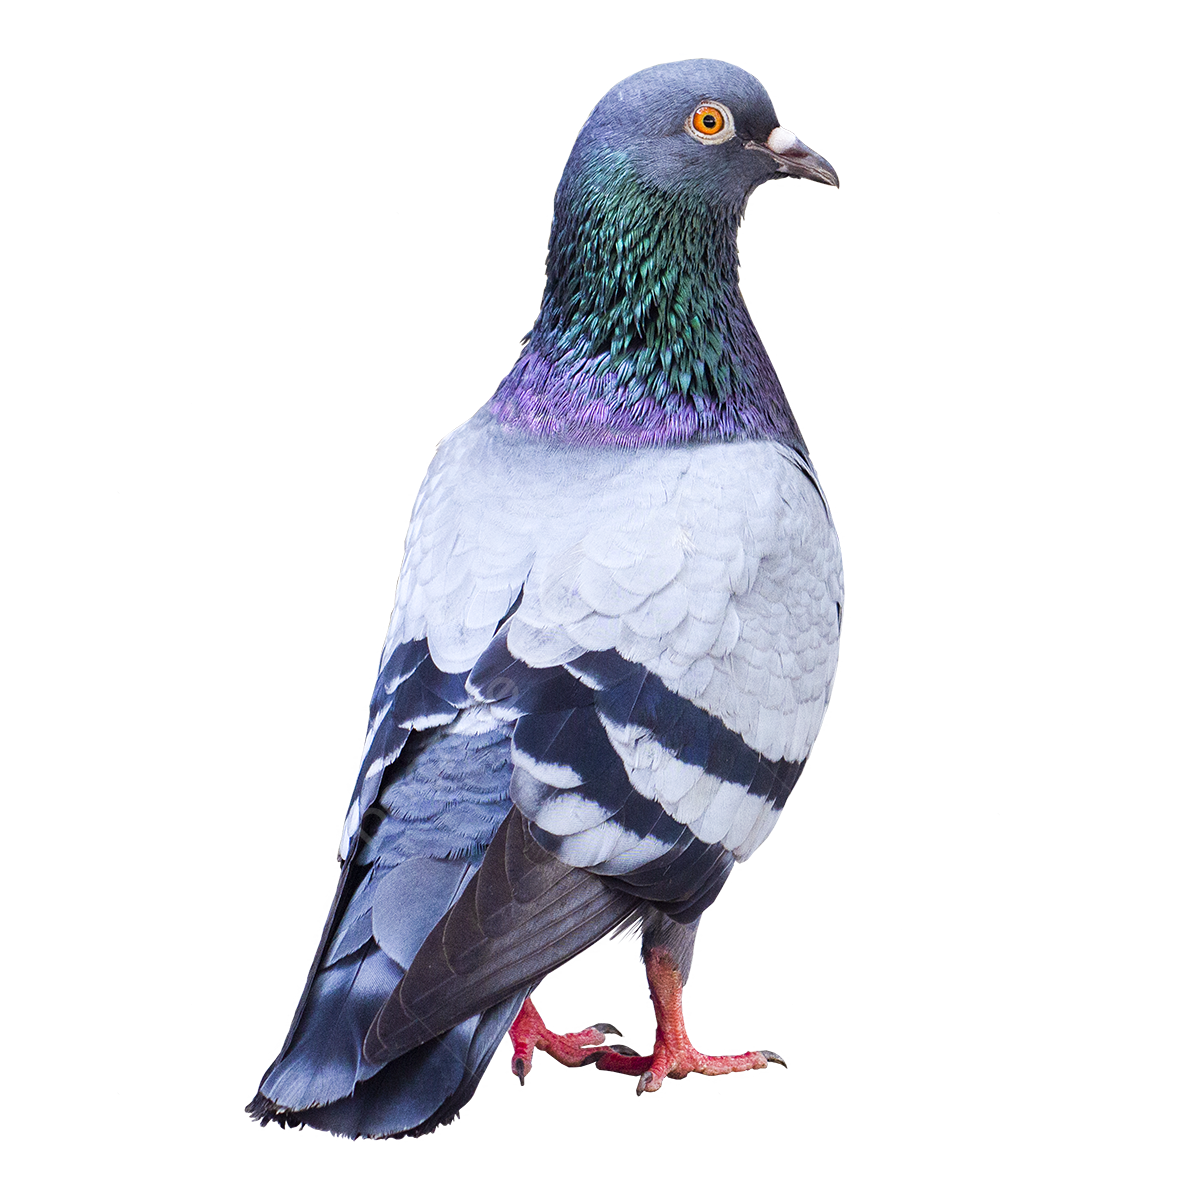
\includegraphics{sample.png}

